\documentclass{beamer}

\usetheme{Madrid} % Or any other theme you prefer
\usepackage[utf8]{inputenc}
\usepackage{amsmath}
\usepackage{amsfonts}
\usepackage{amssymb}
\usepackage{graphicx}
\usepackage{hyperref}
\usepackage{soul}
\usepackage{breqn}

% For code listings, you might need 'minted' or 'listings' package
% For 'minted', you need to compile with pdflatex -shell-escape
%\usepackage{minted}
% Alternatively, for 'listings':
\usepackage{listings}
\lstset{
    language=Python,
    basicstyle=\ttfamily\small,
    numbers=left,
    numberstyle=\tiny,
    stepnumber=1,
    numbersep=5pt,
    tabsize=2,
    extendedchars=true,
    breaklines=true,
    keywordstyle=\color{blue},
    stringstyle=\color{red},
    commentstyle=\color{green!50!black},
    showspaces=false,
    showtabs=false,
    frame=single,
    frameround=tttt,
    backgroundcolor=\color{gray!10}
}


\title{NoProp: Training Neural Networks Without Backpropagation or Forward Propagation}
\author{Presented by Ivan Brillo}
\date{August 1, 2025}
% versione oridinale del codice NoProp: https://github.com/Sid3503/NoProp

\begin{document}

\frame{\titlepage}

\section{Introduction}

\begin{frame}{Introduction: The Deep Learning Dilemma}
    \begin{itemize}
        \item Traditional Neural Network (NN) training relies heavily on:
        \begin{itemize}
            \item \textbf{Forward Propagation:} Computing outputs from inputs.
            \item \textbf{Backpropagation:} Calculating gradients to update weights.
        \end{itemize}
        \item These methods are fundamental but come with significant costs:
        \begin{itemize}
            \item High memory consumption (storing activations for backprop).
            \item Intensive computational requirements.
            \item Complexity, especially as models scale to billions of parameters.
        \end{itemize}
    \end{itemize}
\end{frame}

\begin{frame}{The Rise of Alternative Training Paradigms}
    \begin{itemize}
        \item Growing interest in moving beyond traditional backpropagation.
        \item Motivations include:
        \begin{itemize}
            \item Seeking more biologically plausible learning mechanisms.
            \item Enabling training in constrained environments (IoT/Edge).
            \item Allowing parallel training, that is impossible in traditional approaches due to the sequential propagation of gradients.
        \end{itemize}
        \item NoProp emerges as a radical proposal in this space: \textbf{training neural networks without forward or backward propagation}.

        \begin{itemize}
        \item It treats each layer of the network as a "black box" where only external signals guide learning (input and label embedding).
        \item This flips conventional deep learning on its head by eliminating the need to propagate information end-to-end through the network.
      \item The network's layers don't discover more abstract features of the input as their depth increases; instead, each layer is trained solely to denoise its fixed, noisy input toward the true label embedding.
        \end{itemize}

        
    \end{itemize}
\end{frame}


\section{Understanding NoProp}


\begin{frame}{Forward and Reverse Process in NoProp (1)}

In order to understand how NoProp works, we start by defining:
 \begin{enumerate}
\item $(x, y) \sim q_{data}(x, y)$ our input-lable tuple

\item $z_i \in \mathbb{R}^d$ with $i \in \{1, \dots, T\}$ the \textbf{stochastic} activation of layer $i$ in a neural network, in which each layer has as input the tuple $(x, z_{t-1})$ 
\item $z_0 \sim p(z_0)$ a fixed prior distribution of layer 0 activation
        \end{enumerate}

\medskip

Then we can define, exploiting the chain rule of probabilities and the Markov property: 

 \begin{enumerate}
\item The forward process (generative model)
\[
p_\theta(z_{0:T}, y \mid x)
=
p(z_0) [\, \prod_{t=1}^T p_\theta(z_t \mid z_{t-1}, x) \,] p_\theta(y \mid z_T)
\]

\item The reverse process (variational posterior)
\[
q(z_{0:T} \mid y, x)
=
q(z_T \mid y) \, \prod_{t=1}^T q(z_{t-1} \mid z_t)
\]

        \end{enumerate}


\end{frame}


\begin{frame}{Forward and Reverse Process in NoProp (2)}


\begin{figure}
    \centering
    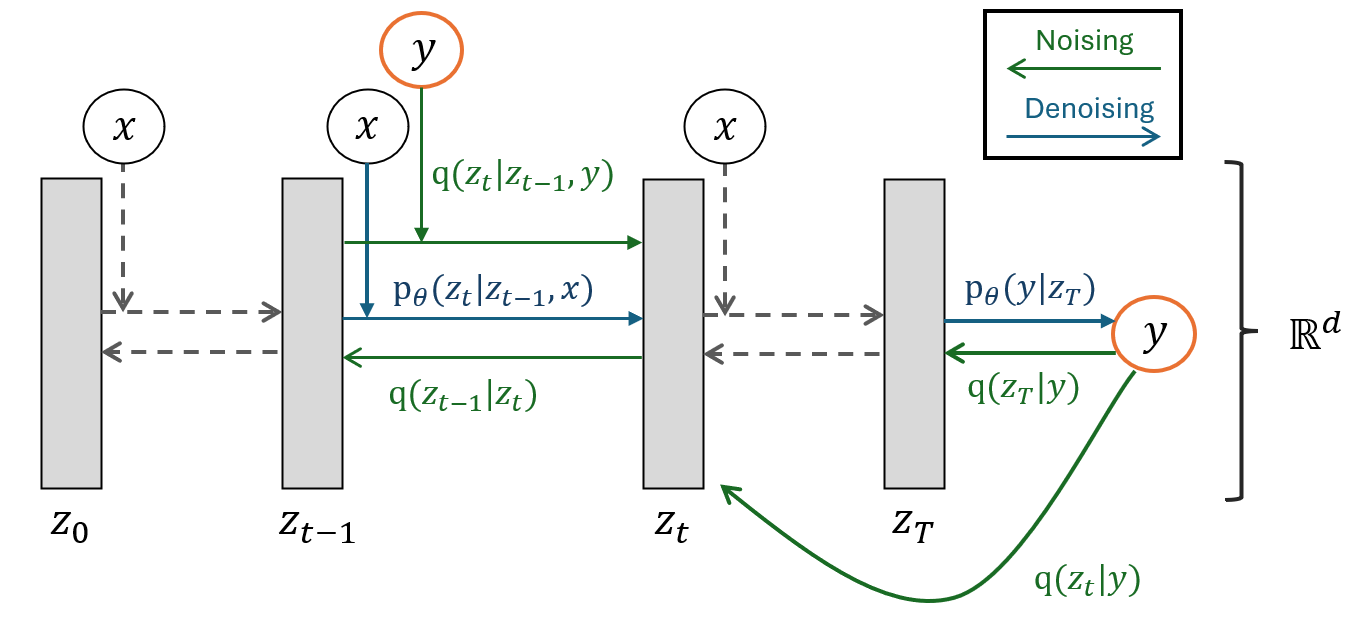
\includegraphics[width=\linewidth]{prob.png}
    \caption{Representation of forward and reverse process in NoProp}
    \label{fig:placeholder}
\end{figure}



\end{frame}

\begin{frame}{Comparison of weight update strategies}


\begin{figure}
    \centering
    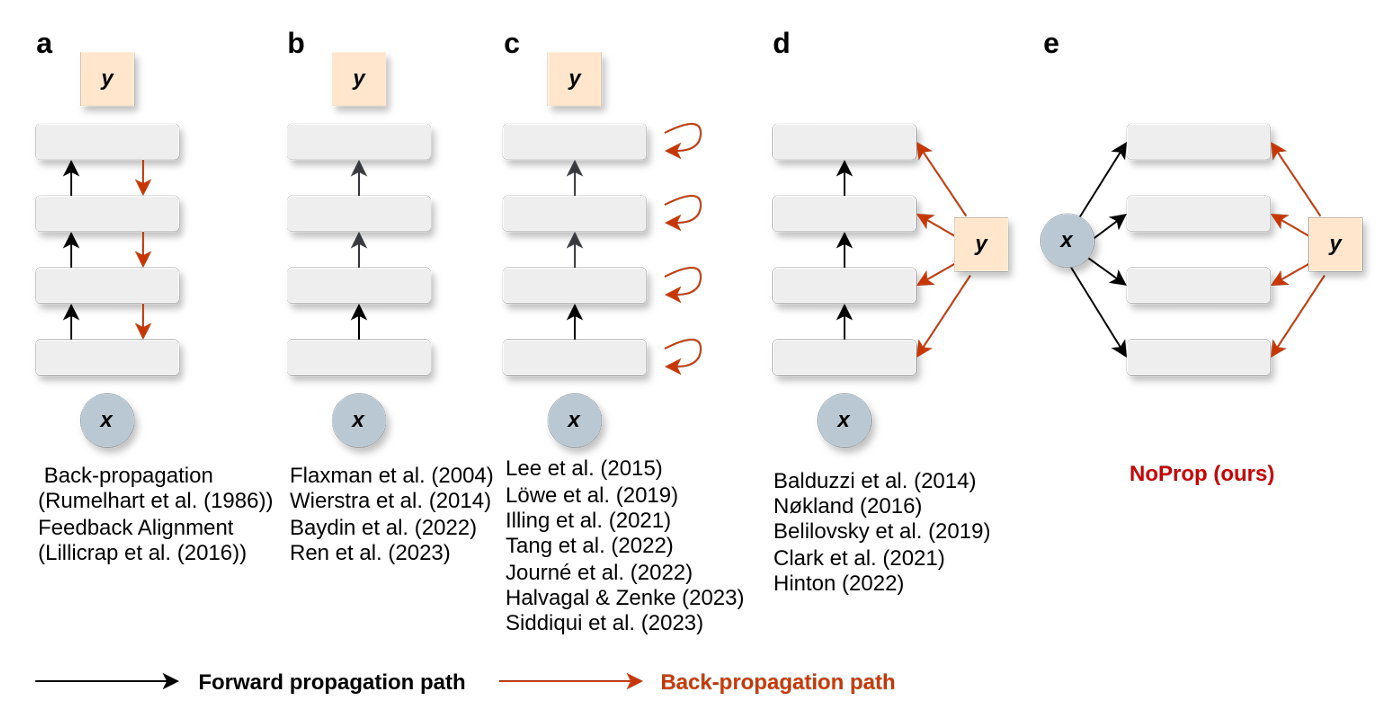
\includegraphics[width=1\linewidth]{comparison.png}
    \caption{ Comparison of weight update strategies in end-to-end back-propagation and its alternatives}
    \label{fig:placeholder}
\end{figure}

\end{frame}


\begin{frame}{Variance Preserving Process}

\textbf{Objective:} Train each \(p_\theta(z_t\mid z_{t-1},x)\) so that, when chained, they "denoise" back to \(y\), without ever propagating \emph{between} layers.

\medskip


The authors fixed the variational posterior to be a tractable Gaussian distribution. Each backward step is defined, as in DDPM, by: 

\[
q(z_{t-1} \mid z_t) = \mathcal{N}\big(\sqrt{\alpha_{t-1}} \, z_t, \, (1-\alpha_{t-1}) I_d\big)
\]

gradually adding noise with a schedule $\alpha_t\in(0, 1)$

\medskip

And, for the last layer:

\[
q(z_{T} \mid y) = \mathcal{N}\big(\sqrt{\alpha_{T}} \, u_y, \, (1-\alpha_{T}) I_d\big)
\]

where $u_y \in \mathbb{R}^d$ is the embedding for class $y$.

\end{frame}


\begin{frame}{Class Embedding}

To represent the discrete class \(y\) as a continuous vector \(u_y\), the authors defined an embedding matrix
\[
W_{\mathrm{EMBED}} \in \mathbb{R}^{d \times c},
\]
where \(c\) is the number of classes and \(d\) is the embedding dimensionality. The class embedding is obtained by selecting the \(y\)-th row of \(W_{\mathrm{EMBED}}\):
\[
u_y = \{W_{\mathrm{EMBED}}\}_y
\]

The embedding matrix \(W_{\mathrm{EMBED}}\) can be either:

\begin{enumerate}
  \item \textbf{Fixed}: for instance, \(W_{\mathrm{EMBED}} = I_c\) (identity matrix) fixing \(d = c\), resulting in a one-hot encoding of classes.
  \item \textbf{Trainable}: \(W_{\mathrm{EMBED}}\) is learned jointly during training (with \(d\) chosen independently of \(c\)), allowing embeddings to capture inter-class similarities (similar to word embeddings in Transformers).
\end{enumerate}

\end{frame}






\begin{frame}{Properties of this Variance Preserving Process (1)}

Defining the variational posterior as we did presents two properties:

\begin{enumerate}
    \item Closed form marginal $ q(z_{t} \mid y) = \mathcal{N}\big(\sqrt{\bar\alpha_{t}} \, u_y, \, (1-\bar\alpha_{t}) I_d\big) $
    with $\bar\alpha_{t} = \prod^T_{s=t} \alpha_s$
\begin{itemize}
    \item $\bar\alpha_{t}$ is strictly increasing. As the number of layers tends to infinity, $q$ collapses to a standard Gaussian, 
    \[
        q(z_{0} \mid y) \;\rightarrow\; \mathcal{N}(0, I_d),
    \]
    since $\bar\alpha_{0}$ is an infinite product of positive terms smaller than one. This property gives $q$ the name \textbf{Variance Preserving} (VP) process, in contrast to Variance Exploding (VE) processes, where the final variance diverges to infinity.

    \item Having a closed-form marginal (which can be interpreted as a discrete Gaussian probability path $q_t$) allows parallel training of the different layers, without requiring forward evaluation. At layer $t$, instead of propagating through the forward process, we can directly sample the previous activation $z_{t-1}$ from the closed-form marginal.
\end{itemize}


\end{enumerate}


\end{frame}




\begin{frame}{Properties of this Variance Preserving Process (2)}

\begin{enumerate}[2]

  \item The process is invertible:
    \[
        q(z_{t} \mid z_{t-1}, y) = \mathcal{N}\big( a_t u_y + b_t z_{t-1}, \; c_t I_d \big)
    \]
    with \(a_t, b_t, c_t\) coefficients computable from \(\{\alpha_{t-1}, \dots, \alpha_T\}\).

\begin{itemize}
\item With the reparameterization trick and substituting $a_t$, $b_t$ and $c_t$, we can write the target stochastic activation of layer \(t>0\) as:
\begin{align*}
z_t^* &= 
\underbrace{a_t u_y}_{\text{label embedding contribution}} +
\underbrace{b_t z_{t-1}^*}_{\text{weighted skip connection}} +
\underbrace{\sqrt{c_t}\,\epsilon}_{\text{Gaussian noise, }\epsilon \sim \mathcal{N}(0,I)} \\
%
&= \frac{\sqrt{\bar\alpha_t} (1 - \alpha_{t-1})}{1 - \bar\alpha_{t-1}} \, u_y
+ \frac{\sqrt{\alpha_{t-1}} (1 - \bar\alpha_t)}{1 - \bar\alpha_{t-1}} \, z_{t-1}^* \\
&\quad + \sqrt{\frac{(1 - \bar\alpha_t)(1 - \alpha_{t-1})}{1 - \bar\alpha_{t-1}}} \, \epsilon.
\end{align*}

\end{itemize}

\end{enumerate}
\end{frame}



\begin{frame}{Loss Formulation (1)}

We want to maximize the log-likelihood of our dataset w.r.t. our model. Unfortunately the value $\log p_\theta(y \mid x) = \log \int p_\theta\bigl(z_{0:T}, y \mid x\bigr) \, d z_{0:T}$ is intractable. Exploiting Variational Inference (VI) we could minimize the negative ELBO:
\[
- \log p_\theta(y\mid x) \le
- \mathbb{E}_{q(z_{0:T}\mid y)}\Big[
\log p_\theta(z_{0:T},y\mid x) - \log q(z_{0:T}\mid y)
\Big] = \mathcal{L}_{\mathrm{NoProp}}
\]

By further simplifying the terms, $\mathcal{L}_{\text{NoProp}}(x, y, \theta)$ becomes: 

\begin{dmath*}
\mathcal{L}_{\text{NoProp}}(x, y, \theta)=
\underbrace{\mathbb{E}_{q(z_T\mid y)}\big[-\log p_{\theta}^{\mathrm{out}}(y\mid z_T)\big]}_{\text{final-step CE}}
+ \underbrace{D_{\mathrm{KL}}\big(q(z_0\mid y)\,\|\,p(z_0)\big)}_{\text{prior KL}}
+ \underbrace{\,
 \sum_{t=1}^T
\mathbb{E}_{q(z_{t-1}\mid y)}
\Big[D_{\mathrm{KL}}\big(q(z_t\mid z_{t-1}, y)\,\|\,p_\theta(z_t\mid z_{t-1}, x)\big)
\Big]}_{\text{denoising error terms}}
\end{dmath*}


\end{frame}


\begin{frame}{Loss Formulation (2)}

Thus, in order to minimize the loss we can impose some restrictions on $p_\theta$ in order to match the same distribution family of the posterior and decrease the complexity of the NN. By looking at $\mathcal{L}$ we can fix:

\begin{enumerate}

\item $p(z_0) = \mathcal{N}(0, I_d)$
\item Since in $q(z_t | z_{t-1}, y)$ the only unknown during inference is $u_y$ we can define $p_\theta(z_t\mid z_{t-1}, x) = \mathcal{N}(a_t\hat u_{\theta _t}(z_{t-1}, x) + b_tz_{t-1} , c_tI_d)$

\medskip


\begin{itemize}

        \item The layer $t$ of the NN needs to learn only an approximation of $u_y$ given $x$ and $z_{t-1}$
        \item The NN doesn't need to estimate the variance of the forward process since it is known apriori
        \item We can express the activation of the NN at layer $0 < t \le T$ as:
        \[
        z_t = 
        \underbrace{a_t \hat u_{\theta _t}(z_{t-1}, x)}_{\text{residual block contribution}} +
        \underbrace{b_t z_{t-1}}_{\text{weighted skip connection}} +
        \underbrace{\sqrt{c_t}\,\epsilon}_{\text{Gaussian noise, }\epsilon \sim \mathcal{N}(0,I)}
    \]
        \item The added noise $\sqrt c_t \epsilon$ contributes to regularize the learning, providing a more robust convergence

\end{itemize}

\end{enumerate}
\end{frame}



\begin{frame}{How $\hat u_{\theta_t}$ is implemented}

\begin{columns}[T] % T aligns the tops of the two columns

  % Right column: text
  \begin{column}{0.5\textwidth}
    $\hat u_{\theta_t}$ is a function that takes as input the previous layer activation $z_{t-1} \in \mathbb{R}^d$ and the input $x \in \mathbb{R}^n$:
    
\[
        \hat u_{\theta_t}: \mathbb{R}^n\times\mathbb{R}^d \rightarrow \mathbb{R}^d
\]    
    
    This function is implemented by a neural network of parameters $\theta_t$. This NN will represent a block of the global neural network, where:
    \begin{itemize}
    \item $T$ layers are present, together with a classification head
      \item Each layer $t$ is defined by the block $\hat u_{\theta_t}(z_{t-1}, x)$
    \end{itemize}
  \end{column}

  % Left column: figure with all float spacing removed locally
  \begin{column}{0.5\textwidth}
    {%
      % locally set float/caption skips to zero so figure doesn't add vertical space
      \setlength{\abovecaptionskip}{0pt}%
      \setlength{\belowcaptionskip}{0pt}%
      \setlength{\intextsep}{0pt}%
      \setlength{\textfloatsep}{0pt}%
      \setlength{\floatsep}{0pt}%
      % small upward nudge if needed (try -1\baselineskip, -0.8\baselineskip, -0.6\baselineskip)
      \vspace{-1.2\baselineskip}%
      \begin{figure}[t] % keep the 't' option
        \centering
        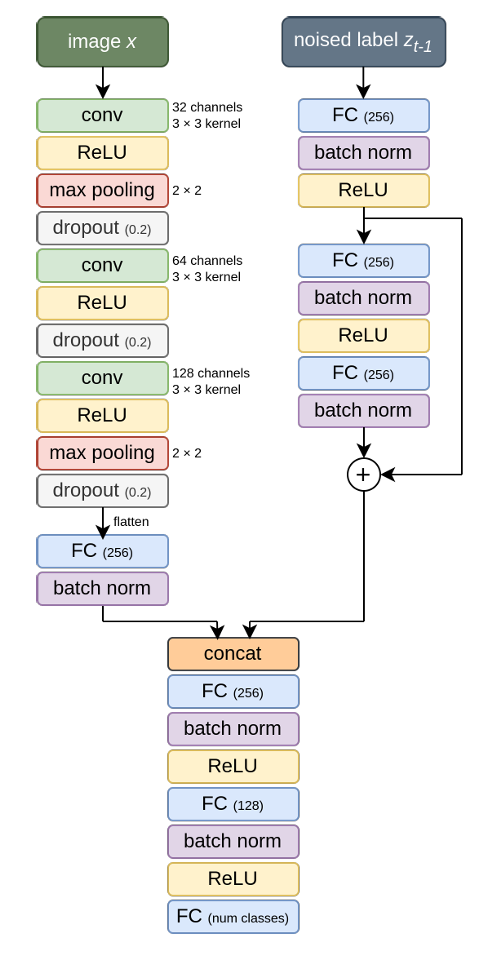
\includegraphics[width=0.6\linewidth]{NN.png}
        \caption{Neural network block used by the authors}
        \label{fig:placeholder}
      \end{figure}%
    }% end local group
  \end{column}

\end{columns}

\end{frame}





\begin{frame}{Loss Formulation (3)}

By further simplifying the loss, we note that the prior KL doesn't depend on $\theta$, and thus can be removed. Substituting the new $p_\theta$ formulation, adding a hyperparameter $\eta$ and calling $\mathrm{SNR}(t) = \frac{\bar \alpha_t}{1-\bar\alpha_t}$


\begin{dmath*}
  \mathcal{L}_{\mathrm{NoProp}}
  = \underbrace{\mathbb{E}_{q(z_T\mid y)}[-\log p_{\theta}^{\mathrm{out}}(y\mid z_T)]}_{\text{final‐step CE}}
  + \underbrace{\tfrac{\eta}{2}\sum_{t=1}^T(\mathrm{SNR}(t)-\mathrm{SNR}(t-1))\,\mathbb{E}_{q(z_{t-1}\mid y)}\big [\|\hat u_{\theta_t}(z_{t-1},x)-u_y\|^2_2 \big]}_{\text{L2 denoising terms}}
\end{dmath*}

\begin{itemize}
    \item $\mathrm{SNR}(t)$ measures how much of the true activation $z_t^*$ comes from true embedding $u_y$ and how much from the injected noise, in fact $ z_{t} \sim \mathcal{N}\big(\sqrt{\bar\alpha_{t}} \, u_y, \, (1-\bar\alpha_{t}) I_d\big) $
\end{itemize}


\end{frame}


\begin{frame}{Key Features of the NoProp Loss}
\begin{enumerate}
  \item {\bf Final‐step cross‐entropy (CE):}
    \[
      \mathbb{E}_{q(z_T\mid y)}\bigl[-\log p_{\theta}^{\mathrm{out}}(y\mid z_T)\bigr]
    \]
    Measures how well the last latent $z_T$ predicts $y$.


  \item {\bf Weighted denoising terms:}
    \begin{itemize}
      \item[$\bullet$] $\big[\mathrm{SNR}(t)-\mathrm{SNR}(t-1) \big] > 0$ weights each denoising step by its signal‐to‐noise gain from the previous layer
      \item[$\bullet$] $\hat u_{\theta,t}(z_{t-1},x)$ is the model's denoiser at layer $t$. It tries to predict the true $u_y$ representation of label $y$.
      \item[$\bullet$] Hyperparameter $\eta$ scales the overall denoising penalty.
    \end{itemize}

  \item {\bf Independence of layer weights} As we can see, all the NN blocks ($p_\theta^{\text{out}}$ and $\hat u_{\theta_t}$) are independent of each other, thus the training can be done independently, without forward or backward propagation

  \begin{itemize}
      \item[$\bullet$] $\nabla_{\theta_x} \hat u_{\theta_t} = 0$  $\forall x \in \{1, \dots, T\} \setminus \{t\}$ similar for $p_\theta^{\text{out}}$ 

\end{itemize}

\end{enumerate}
\end{frame}



\begin{frame}{Training the NoProp Network (DT)}

\textbf{Key Idea:}  
Each layer learns independently to \emph{denoise a noisy target label}, without forward or backward propagation.

\vspace{0.3cm}
\textbf{What is Trained}
\begin{itemize}
  \item Diffusion dynamics blocks $\hat u_{\theta_t}$ (one per timestep $t=1,\dots,T$)
  \item Classifier head $p_{\theta_{\text{out}}}(y|z_T)$
  \item Class embedding matrix $W_{\text{Embed}}$ [optional]
  \item $\text{SNR}(t)$ strictly decreasing noise schedule [optional]
\end{itemize}

\vspace{0.3cm}
\textbf{How Training Works:} for each $(x, y) \in D$ tuple
\begin{enumerate}
  \item For each time step $t \in \{0, \dots, T\}$, sample a noisy activation using the prior $z_{0} \sim \mathcal{N} (0, I_d)$ or the posterior $z_{t} \sim \mathcal{N} (\sqrt{\bar{\alpha}_t}u_y, 1-\bar{\alpha}_t)I_d)$.
  \item Train $\hat u_{\theta_t}(z_{t-1},x)$ to predict the clean embedding $u_y$. Update $\theta_t$.
  \item Train $p_{\theta_{\text{out}}}(y|z_T)$ with cross-entropy loss. Update $ \theta_{\text{out}}$.
\end{enumerate}

\end{frame}


\begin{frame}{Training Considerations}

        The paper uses SGD to train each NN block sequentially but independently.
               \begin{itemize}
        \item This is not mandatory since layers can be updated completely in parallel. Example per internal layer $t \in \{2, \dots, T\}$, repeat until termination condition reached:
        
        \begin{enumerate}
          \item Sample the posterior $z_{t} \sim \mathcal{N} (\sqrt{\bar{\alpha}_t}u_y, 1-\bar{\alpha}_t)I_d)$.
          \item Train $\hat u_{\theta_t}(z_{t-1},x)$ to predict the clean embedding $u_y$. Update $\theta_t$.

\end{enumerate} 
        \end{itemize}
        
        Although not used in the paper, we could train each NN block without computing gradients at all. This could be achieved using techniques inspired by:
        \begin{itemize}
            \item \textbf{Evolutionary algorithms:} Perturbing weights, evaluating fitness (loss impact), and selecting better variants.
        \end{itemize}

\end{frame}

\section{Theoretical Implications and Advantages}


\begin{frame}{NoProp vs. Backpropagation: Key Advantages}
  \begin{enumerate}
    \item \textbf{Memory Efficiency}  
      \begin{itemize}
        \item No need to cache intermediate activations or gradients  
        \item Frees up GPU memory for larger models or higher batch sizes 
        \item Makes training on resource-constrained devices more feasible
      \end{itemize}
    \item \textbf{Immunity to Gradient Pathologies}  
      \begin{itemize}
        \item No vanishing or exploding gradients  
        \item This contributes to more stable and robust training, especially in very deep networks 
      \end{itemize}
    \item \textbf{Massive Parallelism}  
      \begin{itemize}
        \item Unlike backpropagation, which is inherently sequential (gradients flow backward layer by layer), NoProp can update layers concurrently
        \item Greatly accelerates distributed and multi‐device training  
      \end{itemize}

          \item \textbf{Biological Plausibility}  
      \begin{itemize}
        \item Biological neurons are thought to update based on local signals, without a global backpropagation-like mechanism 
        \item Aligns more closely with certain theories of brain-like learning, opening new avenues for neuroscience-inspired AI architectures  
      \end{itemize}
  \end{enumerate}
\end{frame}



%%%%% Slide 1: Flow Matching — Conditional Path & Vector Field %%%%%
\begin{frame}{NoProp-FM: Flow Matching Formulation}
  \begin{itemize}
    \item Let
      \[
        z_0 \;\sim\; p_{\rm init} \;=\;\mathcal{N}(0,I), 
        \qquad
        \mu_{z_1} \;=\; u_y = \{W_{\mathrm{EMBED}}\}_y
      \]
    \item Define a Gaussian conditional probability path, with constant $\sigma^2$
      \[
        p_t(z_t \mid z_0, \mu_{z_1})
        = \mathcal{N}\!\bigl((1-t)z_0 + t\,\mu_{z_1},\;\sigma^2 I\bigr)
        \quad (t\in[0,1]).
      \]
    \item The \emph{true} conditional vector field ($u_t^{\mathrm{target}}$) that given $\mu_{z_1} = u_y$, transforms the noise distribution $p_{init}$ into $\mathcal{N}\!\bigl(\mu_{z_1},\;\sigma^2 I\bigr)$ is given by the following ODE:
    \[
    z_0 \sim p_{\mathrm{init}}, 
    \quad
    \frac{\mathrm{d}}{\mathrm{d}t} z_t = u_t^{\mathrm{target}}(z_t \mid z_0, \mu_{z_1})
    \quad\Longrightarrow\quad
    z_t \sim p_t(\cdot \mid z_0, \mu_{z_1})
    \]
    
    The solution can be simply found using the reparameterization trick and deriving w.r.t. time $z_t = (1-t)z_0+t\mu_{z_1} + \sigma \epsilon$ 
      \[
        u_t^{\mathrm{target}}(z_t\mid z_0,\mu_{z_1})
        = \tfrac{d}{dt}\bigl[(1-t)z_0 + t\,\mu_{z_1}\bigr]
        = \mu_{z_1} - z_0 = u_y - z_0
      \]

      

  \end{itemize}
\end{frame}

%%%%% Slide 2: Flow Matching — Training Objective %%%%%
\begin{frame}{NoProp-FM: Flow Matching Loss}

 Goal: learn a neural vector field \(u_{\theta}(z_t,x, t)\approx u_t^{\mathrm{target}}(z_t\mid z_0,u_y)\).

  \begin{itemize}
    \item Given $(x, y) \sim p_{data}$, sample independently:
      \[
        t\sim U[0,1],\quad
        z_0\sim\mathcal{N}(0,I),\quad
        z_t\sim p_t(z_t\mid z_0,u_y).
      \]
    \item Define the local regression loss
      \[
        \mathcal{L}_{\rm FM}
        = \mathbb{E}_{(x, y), t,z_0,z_t}\;
          \bigl\|\,u_{\theta}(z_t,x, t)\;-\;(u_y - z_0)\bigr\|^2.
      \]
    \item Training occurs by sampling time steps independently, without
 requiring full forward or backward passes through time.

    \item Note that $u_{\theta}(z_t,x, t)$ is a single neural network that takes as input also the time $t$. Thus, the total number of parameters can be much lower than NoProp-DT, sharing them among time.
 
  \end{itemize}
\end{frame}

%%%%% Slide 4: Flow Matching — Sampling (Inference) %%%%%
\begin{frame}{NoProp-FM: Inference Phase}
  \begin{itemize}
    \item After training, the inference problem is solved following the corresponding ODE
      \[
        \frac{\mathrm{d}z_t}{\mathrm{d}t} \;=\; u_{\theta}(z_t,x, t), 
        \quad z_0\sim\mathcal{N}(0,I).
      \]
    \item Discretize the ODE; in this example we will use the Euler method:
      \[
        z_{t+h} = z_t + h\,u_{\theta}(z_t,x,t),\quad h=1/N.
      \]
    \item Simulate the ODE with $N$ timesteps. At \(t=1\), recover $z_1$ and predict:
      \[
        \hat y = \arg\min_{y}\,\|\,z_1 - u_y\|_2^2.
      \]

      \item The paper also presents a formulation of the problem as a continuous diffusion model
  \end{itemize}
\end{frame}



\section{Experimental Results and Performance}

\begin{frame}{Experimental Validation}
    \begin{itemize}
        \item The paper demonstrates NoProp's efficacy on various benchmarks: MNIST, CIFAR-10 and CIFAR-100.
        \item NoProp-DT achieves performance comparable to or better than backpropagation in the discrete-time setting for the same network.

\item A detailed analysis of GPU memory usage between DT and backpropagation confirms a significant memory usage reduction (between 40 and 80\%)
 \begin{itemize}
            \item This makes NoProp highly attractive for Edge Computing and Low-Resource Environments 
\end{itemize}

    \end{itemize}

    \begin{figure}
        \centering
        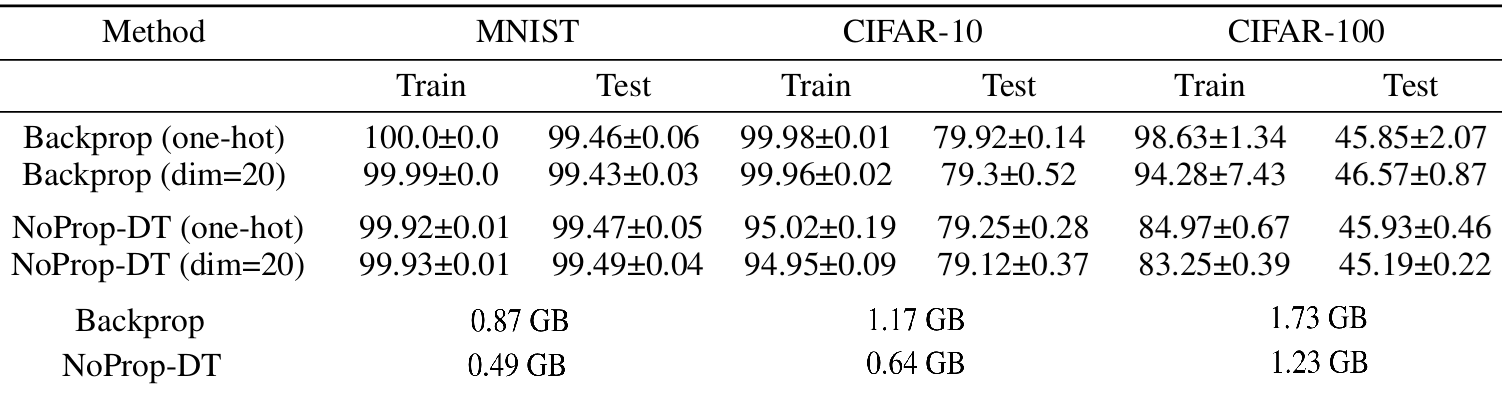
\includegraphics[width=1\linewidth]{Screenshot 2025-08-05 155100.png}
    \end{figure}
\end{frame}


\begin{frame}{Challenges and Limitations}
  \begin{itemize}
    \item \textbf{Limited empirical validation:} NoProp has so far only been demonstrated on small benchmarks (MNIST, CIFAR-10/100) and lacks evaluation on large-scale or real-world datasets.
    \item \textbf{Sensitive hyperparameter tuning:} Although it removes the need for global backpropagation parameters hypertuning, it introduces noise schedules, the embedding matrix, step count as well as all the hyperparameters for the training of each layer
    \item \textbf{Uncertain scaling to deeper models:} By design, each layer learns a local denoising task rather than building hierarchical features; its behavior beyond 10 layers remains untested.
    \item \textbf{Continuous variants lag in accuracy:} In experiments, NoProp-CT and NoProp-FM did not reach the same performance as the discrete-time NoProp-DT variant.
    \item \textbf{Scope limited to classification:} So far the method has only been applied to single-label classification; its adaptation to more complex domains (e.g. NLP) is still open.
  \end{itemize}
\end{frame}


\begin{frame}{References and Code}

\begin{thebibliography}{2}
    \bibitem{ref1} Qinyu Li and Yee Whye Teh and Razvan Pascanu, \emph{NoProp: Training Neural Networks without Back-propagation or Forward-propagation}, 2025.

    \bibitem{ref2} Jonathan Ho, Ajay Jain, Pieter Abbeel, \emph{Denoising Diffusion Probabilistic Models}, 2020.

    \bibitem{ref3} Yaron Lipman, Ricky T. Q. Chen, Heli Ben-Hamu, Maximilian Nickel, Matt Le, \emph{Flow Matching for Generative Modeling}, 2022.

    \bibitem{ref3} Peter Holderrieth and Ezra Erives, \emph{Introduction to Flow Matching and Diffusion Models}, 2025.

    
\end{thebibliography}

\vspace{0.5cm}  % Adds some vertical space



\normalsize  % Reset to normal size

The code implementation of the ideas of the paper can be find:
\begin{itemize}
    \item \href{https://github.com/ivanbrillo/NoProp/blob/main/NoProp.ipynb}{Here}, a simple classification task of MNIST dataset
    % versione originale: https://github.com/Sid3503/NoProp
    \item \href{https://github.com/ivanbrillo/NoProp/blob/main/NoProp_TimeSeries.ipynb}{Here}, a  time series predictor, embedding the network inside an AE
    
\end{itemize}


\end{frame}





\end{document}